\chapter{ИССЛEДОВАТЕЛЬСКАЯ ЧАСТЬ}
\label{cha:ch_2}

В данной части рассматривается моделирование полёта ПТУР с носителя с поражением предполагаемой цели в верхнюю проекцию. Также проводится оценка эффективности поражения цели по критерию минимального угла поражения к нормали и исследование оптимальных, с учетом используемого закона наведения, участков зоны пуска.

\section{Постановка задачи исследования}
Исходными данными для задачи являются:

\begin{enumerate}[1.]
	\item Массовые и баллистические параметры ПТУР;
	\item Располагаемая перегрузка ПТУР;
	\item Параметры головки самонаведения ПТУР;
	\item Диапазон применения БПЛА по высоте;
	\item Параметры средств ПВО противника.
\end{enumerate}

На основании этих данных требуется обосновать возможность построения траектории ПТУР, обеспечивающей поражение целей в верхнюю проекцию.

\section{Комментарии к постановке задачи}
В данном исследовании под ПВО противника принимается 12.7-мм пулемет вида Browning M2 или ДШК, так как ударно-разведывательные БПЛА в настоящее время применяют после подавления основных сил ПВО противника. Максимальная дальность прицельного выстрела у этих пулеметов составляет порядка 2.5 км.

Диапазон применения БПЛА по высоте принимается отрезком от 500 до 4000 м.

В качестве ПУТР был принят лёгкий ПТУР, проектируемый для запусков с БПЛА и разрабатываемый в рамках курсового проекта. Максимальная поперечная перегрузка ПТУР, поражение которым исследуется, составляет 6G. Головка самонаведения применяемого ПТУР – полуактивная лазерная. Угол захвата ГСН принимается 60 градусов.

Предполагается, что данные о законе перегрузки, о котором речь пойдет в следующем параграфе, вводятся в ПТУР при пуске на основании данных о дальности до цели и характере её передвижения, получаемых и обрабатываемых СУ БПЛА.

\section{Подход к алгоритму решения}
Идеальной траекторией для поражения цели была бы траектория, представленная на рисунке \ref{fig:ideal_traec}.

\begin{figure}[h]
\begin{center}
	\begin{minipage}[h]{0.47\linewidth}
		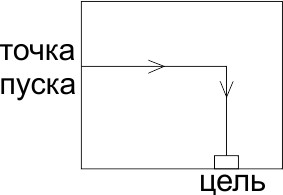
\includegraphics[width=1\linewidth]{ideal_traek}
		\caption{Идеализированная траектория для поражения цели сверху}
		\label{fig:ideal_traec}
	\end{minipage}
	\hfill
	\begin{minipage}[h]{0.47\linewidth}
		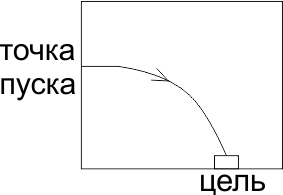
\includegraphics[width=1\linewidth]{real_traec}
		\caption{Реальная траектория для поражения цели сверху}
		\label{fig:real_traec}
	\end{minipage}
\end{center}
\end{figure}

Однако траектория такого вида недостижима для реальных ПТУР, так как для любых реальных ЛА существуют ограничения по перегрузке, не позволяющие так резко менять курс. Таким образом, переходим к следующему варианту траектории, представленному на рисунке \ref{fig:real_traec}.

Данная траектория достижима на практике. Однако при использовании полуактивной ГСН головка должна постоянно держать цель в своем угле обзора. Таким образом, накладывается ограничение на вид траектории, и она принимает вид как на рисунке. На рисунке \ref{fig:with_gsn} угол захвата ГСН показан пунктирными линиями.

\begin{figure}[h]
\begin{center}
	\begin{minipage}[h]{0.47\linewidth}
		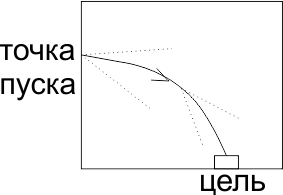
\includegraphics[width=1\linewidth]{with_gsn}
		\caption{Траектория с учётом угла захвата ГСН}
		\label{fig:with_gsn}
	\end{minipage}
	\hfill
	\begin{minipage}[h]{0.4\linewidth}
		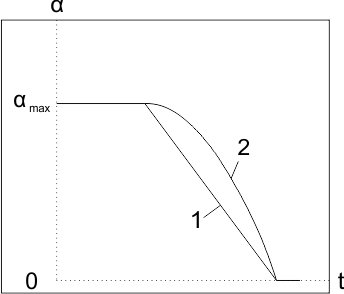
\includegraphics[width=1\linewidth]{peneng_function}
		\caption{Варианты функций изменения пеленга}
		\label{fig:peleng_function}
	\end{minipage}
\end{center}
\end{figure}

Для реализации такого манёвра используется следующий закон наведения: на начальном этапе между вектором скорости ПТУР и линией, соединяющей ПТУР и цель, есть угол. Этот угол, называемый углом пеленга, на активном участке полета принимает максимальное значение. Далее, при приближении к цели, этот угол уменьшается, в идеале приходя в нуль при встрече с целью. В данной работе угол пеленга обозначается $\alpha$.

В простейшем идеальном случае изменение угла пеленга происходит скачкообразно из максимального значения в минимальное. Однако этот скачок вызывает также скачок перегрузки, что недопустимо. Также не подходит линейное изменение угла пеленга, так как в начале линейного участка ПТУР также испытывает скачкообразную перегрузку.

В данной работе угол меняется от максимального значения до минимального по квадратичному закону. Это позволяет плавно наращивать перегрузку в начале маневра. Отсутствие перегиба, возникающего при использовании функций более высокого порядка, обеспечивает плавный рост перегрузки в оставшейся части маневра.

Функции пеленга с линейным изменением угла $\alpha$ (1) и с изменением по квадратичному закону (2) показаны на рисунке \ref{fig:peleng_function}.

Далее, после определения вида функции, встает вопрос о длине отрезка манёвра и расположении его между началом полета и временем встречи. На рисунке \ref{fig:peleng_x_traec} показаны два варианта траектории с разной длиной манёвра. Можно заметить, что траектория 2, которой соответствует меньшее время маневра, более крутая и более вертикально встречается с целью при том, что точка пуска в обоих случаях одинакова.

\begin{figure}[!h]
\begin{center}
	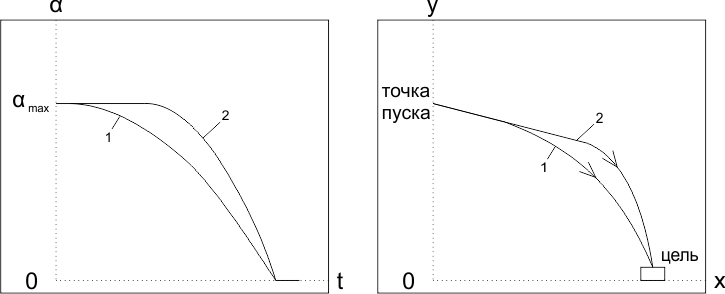
\includegraphics[height=65mm]{peleng_x_traec}
	\caption{Влияние изменения пеленга на вид траектории}
	\label{fig:peleng_x_traec}
\end{center}
\end{figure}Для определеня успешности поражения цели введем угол встречи с целью, отложенный от вертикали. В данной работе этот угол обозначается $\gamma$. Визуально этот угол показан на рисунке \ref{fig:meeting_angle}.

\begin{figure}[!h]
\begin{center}
	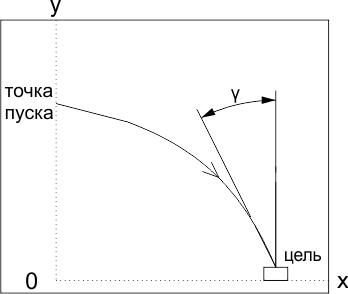
\includegraphics[height=70mm]{meeting_angle}
	\caption{Угол встречи с целью}
	\label{fig:meeting_angle}
\end{center}
\end{figure}

Соответственно, чем угол $\gamma$ меньше, тем лучше бронепробитие ПТУР и более успешно поражается цель. С другой стороны, если обратиться к рисунку \ref{fig:peleng_x_traec} с траекториями, ракета на траектории 2 будет испытывать большие перегрузки из-за более резкой смены курса. 

\clearpage
Итак, возникает задача оптимизации:
\begin{enumerate}[1.]
	\item Задано расстояние до цели L и высота пуска H;
	\item Известен вид закона изменения пеленга $\alpha (t)$;
	\item Требуется найти время начала и конца маневра, $t_\text{нач}$ и $t_\text{кон}$ соответственно, такие что угол встречи с целью $\gamma$ минимален и при этом максимальная испытываемая перегрузка $n_{max} ≤ n_\text{расп}$.
\end{enumerate}

Данную задачу возможно решить перебором большого количества точек пуска и получить поверхность с углами $\gamma$.

\section{Описание алгоритма решения} \label{chapter:traectory_optimization}
Для решения данной задачи используется следующий алгоритм.
\begin{enumerate}[1.]
	\item Пространство пуска ПТУР разбивается по высоте и дальности на отрезки длиной 100 м.
	\item Каждая точка получившейся сетки поочередно принимается точкой пуска ПТУР. 
	\item Находится начальное приближение длительности манёвра и времени его завершения. Для этого решается задача полета для ПТУР с прямолинейной траекторией, наводящегося на активном участке с максимальным пеленгом, а на пассивном по методу чистой погони. Таким образом, угол пеленга гарантированно придет в нуль до встречи с целью, если полученное $t_\text{кон}$  использовать в представленном на рисунке 4 законе наведения. 
	\item Длительность манёвра итерационно уменьшается при сохранении конечной точки манёвра по времени. На каждой итерации снова решается задача полета ПТУР, определяется угол встречи с целью $\gamma$ и максимальная испытываемая перегрузка $n_{max}$. Остановка процесса происходит либо при превышении максимальной испытываемой перегрузки, либо при достижении значения угла $\gamma$ менее 5°.
	\item Для точки каждой пары дальности и высоты находится значение $\gamma$. На основании этого возможно сделать вывод об оптимальной области пуска ПТУР.
\end{enumerate}

Визуально шаги расчёта представлены на рисунке \ref{fig:visual_optimize}. Там шаг 0 – получение $t_\text{кон}$, далее шаги 1, 2, 3 – последовательное увеличение $t_\text{нач}$ , приводящее к уменьшению угла $\gamma$ и увеличению испытываемых перегрузок.
\begin{figure}[!h]
\begin{center}
	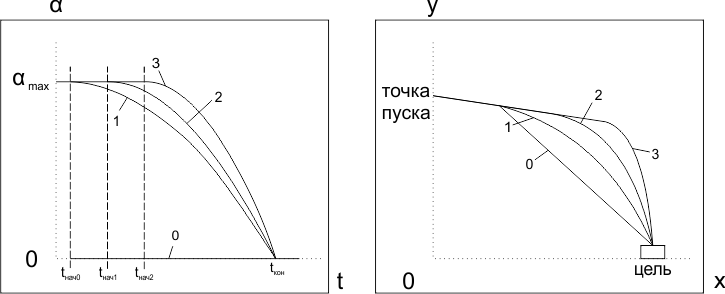
\includegraphics[height=70mm]{visual_optimize}
	\caption{Визуальная интерпретация оптимизации\\ закона изменения пеленга}
	\label{fig:visual_optimize}
\end{center}
\end{figure}

\section{Описание математической модели}
В целом, для реализации описанного выше алгоритма требуется решить следующие математические задачи:
\begin{enumerate}[1.]
	\item Решение задачи полета ПТУР (построение траектории и диаграммы скорости) при известных параметрах пуска и характеристиках ракеты;
	\item Нахождение перегрузки на траектории.
\end{enumerate}

\subsection{Решение задачи полета ПТУР}
Для решения задачи на активном и пассивном участках используется системы уравнений (\ref{system:active}) и (\ref{system:passive}), приведенные на странице \pageref{system:active}.

В данной работе рассматривается квадратичный закон изменения угла пеленга, поэтому в этих системах уравнений закон $\alpha(t)$ имеет вид, описанный в уравнении (\ref{system:nice_alpha}).

\begin{equation}
	\label{system:nice_alpha}
	\alpha(t) = \begin{cases}
		\alpha_{max} & \text{, если t < } t_\text{нач} \\
		\alpha t^2 + 2bt + c &  \text{, если } t_\text{нач} \le t < t_\text{кон} \\
		0 &  \text{, если t } \ge t_\text{кон}
	\end{cases}
\end{equation}
Коэффициенты $a, b, c$ введены для удобства записи, они выражаются как:
\begin{align*}
a & = \frac{\alpha_{max}}{ (t_\text{нач}^2 - t_\text{кон}^2) - 2(t_\text{нач}^2-t_\text{нач} t_\text{кон}) } \\
b & = -2 \alpha t_\text{нач} \\
c & = \alpha_{max} - \alpha t_\text{нач}^2 - b t_\text{нач}
\end{align*}

Здесь $t_\text{нач}$ - время начала манёвра; $t_\text{кон}$ - время завершения маневра; $\alpha_{max}$ - максимальный угол пеленга (параметр ГСН).

\clearpage
\subsection{Нахождение перегрузки, действующей на ЛА}
Угол атаки ЛА в полете принимается постоянным.

В каждой точке мы знаем значение модуля скорости ЛА, а также скорость и координаты этой точки в последующей и предыдущей точках интегрирования (кроме первой и последней). Таким образом, можно узнать перегрузку в точке, построив вектора скорости до неё и после неё. Далее можно найти поперечную составляющую изменения скорости, и, поделив на соответствующий отрезок интегрирования, поперечную перегрузку.

Графическая иллюстрация алгоритма представлена на рисунке \ref{fig:visual_overload}.
\begin{figure}[!h]
\begin{center}
	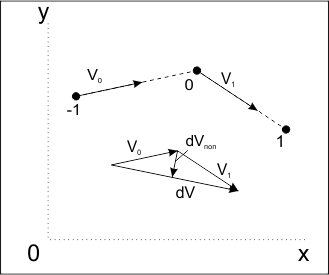
\includegraphics[height=70mm]{visual_overload}
	\caption{Визуальная интерпретация поиска\\ перегрузки на траектории}
	\label{fig:visual_overload}
\end{center}
\end{figure}

\clearpage
\section{Описание реализации алгоритма}
Поставленная задача численно решается с помощью языка программирования Python второй версии. Помимо стандартной библиотеки в реализации используются следующие компоненты:
\begin{enumerate}[1.]
	\item Numpy
	\item Matplotlib
	\item Scipy
\end{enumerate}

Также в исходный код системы включен компонент Python Progress Bar, исходный код которого взят по адресу: \url{https://gist.github.com/aubricus/f91fb55dc6ba5557fbab06119420dd6a}.

Каждый из компонентов системы является свободно распространяемым и предоставляется авторами бесплатно. Таким же образом распространяется и код, решающий поставленную задачу. При возникновении интереса, его можно найти по адресу, записанному в приведенном на рисунке \ref{fig:qr_code} QR-коде, а также установить на собственный компьютер. Там же можно задать вопросы автору кода.

\begin{figure}[!h]
\begin{center}
	
\includegraphics[height=70mm]{qr_code}
	\caption{QR-код для перехода в репозиторий}
	\label{fig:qr_code}
\end{center}
\end{figure}

На рисунке \ref{fig:program_scheme} представлено дерево файлов и схема зависимостей программной реализации.

\begin{figure}[!h]
\begin{center}
	\includegraphics[width=\linewidth]{program_scheme}
	\caption{Схема файлов и зависимостей программы}
	\label{fig:program_scheme}
\end{center}
\end{figure}

Так как python – интерпретируемый язык программирования, все исходные тексты программы могут быть изучены и отредактированы для реализации нового функционала непосредственно перед запуском без необходимости дополнительной рекомпиляции кода.

Для хранения констант и всех вариаций координат точки старта ПТУР используются файлы формата .pkl. Эти файлы создаются и читаются с помощью модуля pickle, входящего в стандартную библиотеку python.

\subsection{Установка и запуск системы}
\begin{enumerate}[1.]
	\item Установить Python второй версии, не старше версии 2.7.
	\item Установить перечисленные выше компоненты системы (предпочтительно – с помощью пакета pip)
	\item Клонировать приведенный выше репозиторий или загрузить оттуда исходный код и разархивировать.
	\item В папке const/ проекта отредактировать файлы missile\_const.py и bearing\_styles.py в соответствии с рассматриваемой задачей.
	\item Запустить поочередно файлы .py из папки const
	\item Открыть файл make\_start\_mesh.py, ввести желаемый разброс координат пуска ПТУР. Для корректной работы отображения итоговой поверхности рекомендуется выбирать точки с шагом 100 метров.
	\item Запустить файл make\_start\_mesh.py
	\item Запустить файл traectory\_variation.py. Его исполнение может занять некоторое время, прогресс выполнения выводится в консоль в виде статус-бара (см рисунок \ref{fig:run_example})
	\item Запустить файл graphics/create\_wire\_map.py и изучить полученную поверхность. 
\end{enumerate}

\begin{figure}[!h]
\begin{center}
	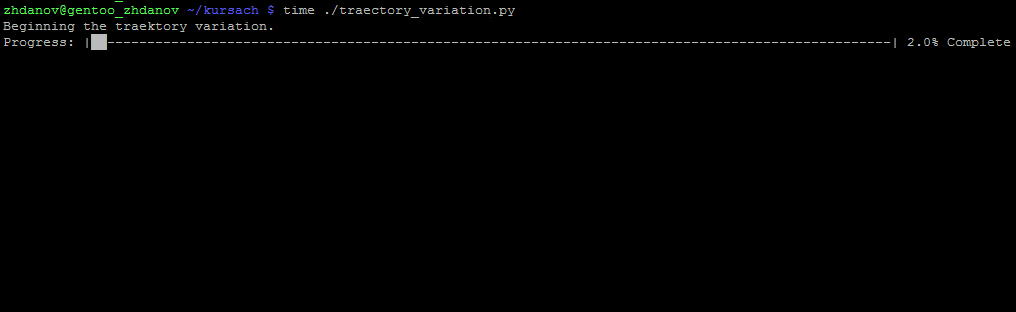
\includegraphics[width=\linewidth]{run_example}
	\caption{Пример консольного вывода основного расчета}
	\label{fig:run_example}
\end{center}
\end{figure}

Также для отладки нового функционала или валидации результатов расчета возможно использовать файл one\_traectory\_variation.py. Этот функционал проводит оптимизацию траектории для одной стартовой точки. После выполнения, результат работы программы (траекторию) можно визуально посмотреть, запустив graphics/show\_traectory.py.

Пример вывода траектории полета представлен на рисунке \ref{fig:one_picture_example}.
\begin{figure}[!h]
\begin{center}
	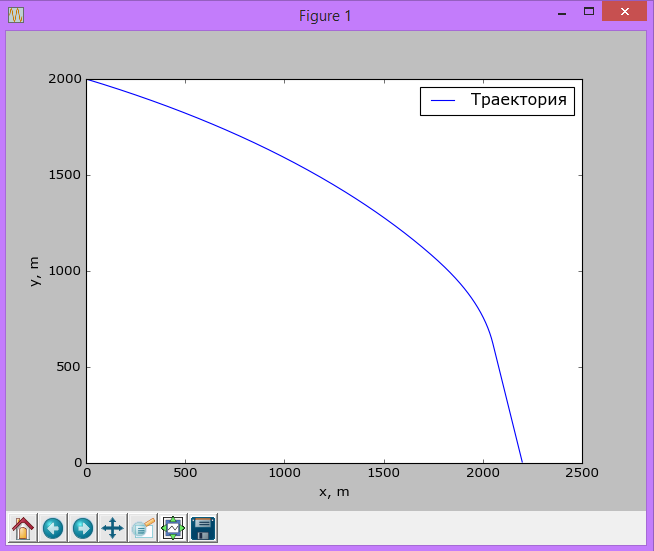
\includegraphics[width=0.7\linewidth]{one_picture_example}
	\caption{Пример вывода основного расчета}
	\label{fig:one_picture_example}
\end{center}
\end{figure}


\clearpage
\section{Результат работы}
В результате работы создана программа, способная циклически выполнять алгоритм, описанный выше и создавать массив в данными о угле поражения цели в разных точках пуска. Все части алгоритма реализованы с помощью открытых средств разработки для языка программирования Python.

Также разработан алгоритм представления полученных результатов в виде поверхности. Так как это трехмерная поверхность, в этом отчете представлено несколько проекций фигуры на рисунках \ref{fig:result_1}, \ref{fig:result_2} и \ref{fig:result_3}.

\begin{figure}[!h]
\begin{center}
	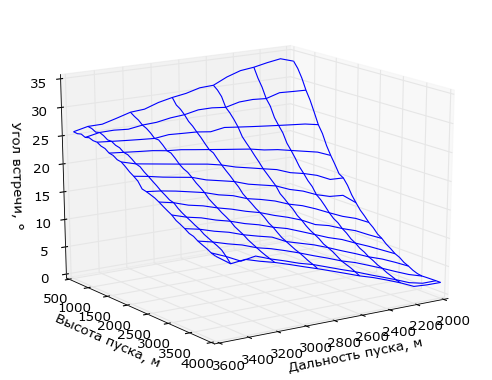
\includegraphics[width=\linewidth]{result_1}
	\caption{Представление результата исследования}
	\label{fig:result_1}
\end{center}
\end{figure}

\begin{figure}[!h]
\begin{center}
	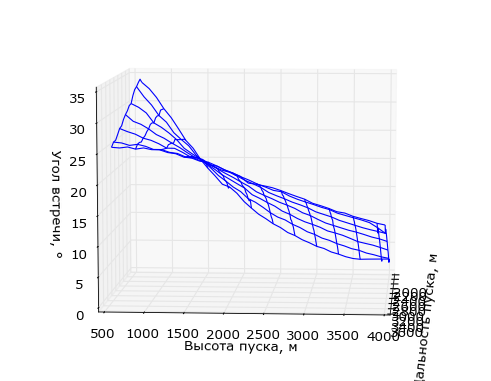
\includegraphics[width=0.8\linewidth]{result_2}
	\caption{Представление результата исследования}
	\label{fig:result_2}
\end{center}
\end{figure}

\begin{figure}[!h]
\begin{center}
	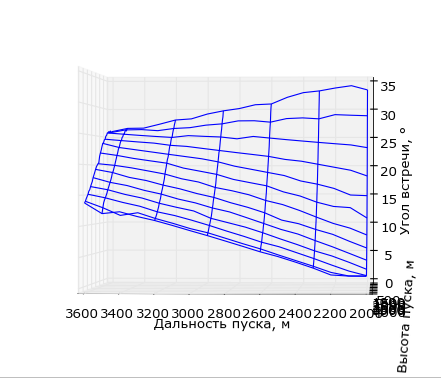
\includegraphics[width=0.8\linewidth]{result_3}
	\caption{Представление результата исследования}
	\label{fig:result_3}
\end{center}
\end{figure}

\clearpage
\section{Результат исследования}
В результате данной работы обоснована возможность применения используемого алгоритма для построения траектории для поражения целей в верхнюю полусферу. В результате, угол встречи с целью $\gamma$ при стрельбе из любой точки пуска рассматриваемой области оказался в пределах 35°, что является удовлетворительным результатом, так как большинство современных систем активной защиты не защищают от снарядов, летящих под такими углами.

Также на основании полученного результата, можно сделать следующие выводы:
\begin{enumerate}[1.]
 	\item Угол поражения в большей степени зависит от высоты пуска ПТУР, чем от горизонтальной дальности до цели. Если изменение угла встречи по дальности носит приблизительно линейный характер, но изменение по высоте выражается более выпуклой функцией. При выборе точке пуска из вариантов с одинаковой горизонтальной дальностью выгоднее запускать ПТУР с большей высоты.
 	\item Наилучшие результаты по углу встречи оказались в точках с минимальной дальностью пуска и максимальной его высотой.
 	\item Порядка четверти всей зоны пуска ПТУР позволяет поражать цель с углом встречи не более 15°, что является хорошим результатом, так как в этом случае реальное бронепробитие менее чем на 5\% упадет по сравнению с бронепробитием по нормали.
\end{enumerate}
